\documentclass[a4paper]{template/imereport}
\usepackage[utf8]{inputenc}
\usepackage{ucs}
\usepackage[ngerman]{babel}
\usepackage{graphicx}
\usepackage{wrapfig}
\usepackage{listings}
\usepackage[T1]{fontenc}
\usepackage[scaled]{beramono}

\usepackage{color}
\definecolor{bluekeywords}{rgb}{0.08,0.08,0.5}
\definecolor{greencomments}{rgb}{0,0.5,0}
\definecolor{redstrings}{rgb}{0.9,0,0}
\lstset{ %
    captionpos=b,
    breaklines=true,
    basicstyle=\footnotesize\ttfamily,
    frame=single,
    keywordstyle=\color{bluekeywords}\bfseries,
    morekeywords={proc, pure, ensures, requires, call, in, out, var, const ,init, fun, copy, ref, while, returns, if, else}
}

\pagestyle{myheadings}
\markboth{IML Compiler}{IML Compiler}

% Title section
\author{Florian Lüscher, Matthias Brun\\
Fachhochschule Nordwestschweiz\\
\small{\texttt{<\{florian.luescher,matthias.brun\}@students.fhnw.ch>}}
}
\title{IML Compiler: Enhancements for Robust Programming}

\begin{document}

\maketitle

% Einleitung
Obwohl in den vergangenen Jahrzehnten im Bereich des Softwareengineerings viel 
Aufwand in das Entwickeln von Technologien zur effizienteren Entwicklung robuster
Software gesteckt wurde, gibt es noch immer wenige Programmiersprachen welche 
das Schreiben robuster Software beim Sprach-Design berücksichtigt haben. Eine der Ausnahmen 
ist die Sprache Eiffel, welche beispielsweise das Definieren von Pre-/Postconditions
ermöglicht. Jedoch gibt es vermehrt auch Frameworks für etabliertere Sprachen, welche 
es erlauben, Elemente des Design-by-Contract anzuwenden und vom Compiler zu überprüfen.
In der Sprache C\# von Microsoft beispielsweise wird dies mittels \textit{Code Contracts}
 ermöglicht, welche auch vom Compiler statisch analysiert werden \cite{MS:CodeContracts}.
Auf der Java Platform gibt es über den Community Process Anstrengungen, über Annotationen
zusätzliche Metainformationen bereitszustellen, welche von einem externen Tool (z.B. FindBugs) statisch analysiert 
werden können und den Programmierer bei möglichen Fehlern warnen \cite{JSR:305}. Jedoch wurde dies
auch im aktuellen Compiler der Java Version 7 noch nicht implementiert werden. In diesem Bericht werden Erweiterungen
der Unterrichtsprache IML beschrieben, welche das Schreiben robuster Software erleichtern sollen.



% Inhalt
\section{Ausgangslage}

Als Grundlage wird das Sprachdesign von IML dienen, wie es zur Verfügung gestellt wurde. In einer ersten 
Phase wurde ein Compiler für diesen Sprachumfang entwickelt, welcher danach für die in diesem Dokument
beschriebenen Erweiterungen angepasst wurde. Dieser Compiler wurde auf Basis der Sprache Scala entwickelt,
da diese einerseits funktionale Aspekte beim Programmieren ermöglicht, andererseits bereits 
Parser-Kombinatoren im Sprachumfang enthalten sind.


\newpage

%\begin{figure*}[h]
%	\begin{center}
%		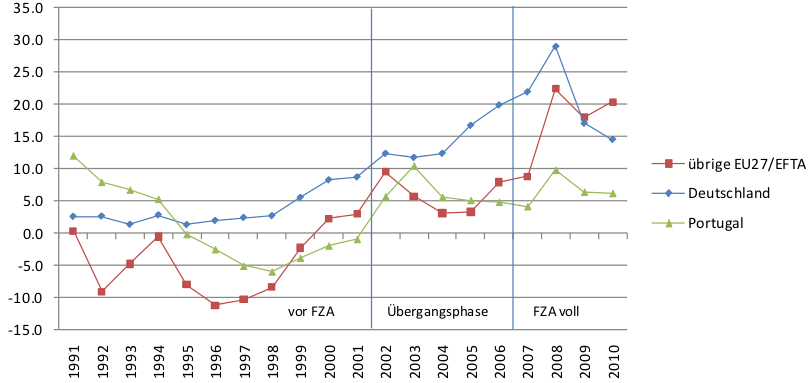
\includegraphics[width=0.9\textwidth]{images/Zuwanderungssaldo_Bericht_2.png}
%	\end{center}
%	\caption{Verlauf der Zuwanderung nach Herkunftsländern in Tausend \cite[S. 18]{ADMIN:Bericht}}
%	\label{fig:zuwanderungsaldi}
%\end{figure*}


%\section{Parser-Architektur}

Kurze Beschriebung der Architektur mit Diagramm


%\newpage

%\begin{figure*}[h]
%	\begin{center}
%		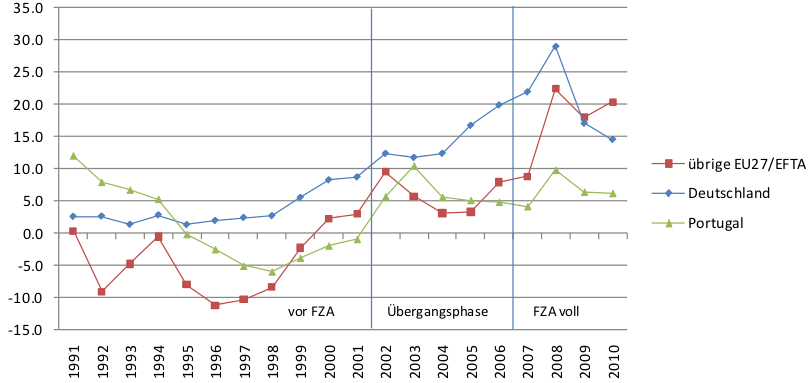
\includegraphics[width=0.9\textwidth]{images/Zuwanderungssaldo_Bericht_2.png}
%	\end{center}
%	\caption{Verlauf der Zuwanderung nach Herkunftsländern in Tausend \cite[S. 18]{ADMIN:Bericht}}
%	\label{fig:zuwanderungsaldi}
%\end{figure*}


\section{Spracherweiterungen}
In diesem Abschnitt werden die geplanten Erweiterungen an der Sprache erläutert. 
Ein wichtiges Kriterium für unsere Erweiterungen war es, die Kompatibliität von 
zur Standard-IML beizubehalten. Es muss möglich sein, bereits vorhandene Programme
auch mit dem erweiterten Compiler zu kompilieren und eine äquivalentes Programm zu 
erhalten. Dies macht es zudem leichter, bestehende IML Programme um pre-/postconditions
zu erweitern.
Die vollständige Grammatik der Sprache ist im Anhang \ref{sec:fullgrammar} 
ersichtlich. Weitere funktionierende sowie nicht funktionierende beispiele sind in den Anhängen
\ref{sec:good_examples} und \ref{sec:bad_examples} zu finden.

\subsection{Pre-/Postconditions}
Das definieren von pre- und postconditions sollte direkt beim Deklarieren
der Prozedur oder der Funktion ermöglicht werden. So sind die Garantien
für den Programmierer auf einen Blick ersichtlich und erleichern so 
das Verständnis der Prozedur. In Listing \ref{lst:first} ist ein Beispiel 
einer Prozedur mit conditions ersichtlich. Das Label "dump\_condition" dient dazu, im
Falle eines Fehlschlags der darauffolgenden condition hilfreiche Fehlermeldungen generieren zu können.
In Folge des Fehlens eines String-Literals wird ein Ident verwendet.
Als conditions können alle Expressions verwendet
werden, welche zu einem boolean Typ ausgewertet werden. Mehr dazu wird im 
Kapitel \ref{sec:constraints} erleutert.
\newline
\begin{lstlisting}[caption=Beispiele von pre-/postconditions,label={lst:first}]
proc divide(in copy m:int32, in copy n:int32, out ref q:int, out ref r:int32)
requires [n > 0, dumb_condition: unnecessary(m, n)]
ensures [r >= 0]
{
    q init := 0;
    r init := m;

    while(r >= n) {
        q := q+1;
        r := r-n;
    }
}
\end{lstlisting}

\subsubsection{Lexikalische Syntax}
Es wurden die in Listing \ref{lst:terminals} ersichtlichen neuen Terminale eingeführt.
\begin{lstlisting}[caption=Liste neuer Terminalsymbole,label=lst:terminals]
[           (Token: LBRACKET)
]           (Token: RBRACKET)
requires    (Token: REQUIRES)
ensures     (Token: ENSURES)
\end{lstlisting}

%\newpage
\subsubsection{Grammatikalische Syntax}
Die Grammatik wurde um neue nichtterminal Symbole erweitert. Zudem wurden die NTS funDecl und 
procDecl erweitert, damit nun die conditions an die Deklaration gehängt werden können. Die angepassten
Symbole sind in Listing \ref{lst:decls} dokumentiert.
\newline
\begin{lstlisting}[caption=Neue nichtterminal Symbole]
requires        ::= REQUIRES conditionList
ensures         ::= ENSURES  conditionList

conditionList   ::= LBRACKET [condition {COMMA condition}] RBRACKET
condition       ::= [IDENT COLON] expr

\end{lstlisting}

\begin{lstlisting}[caption=Angepasste nichtterminal Symbole,label=lst:decls]

funDecl     ::= FUN IDENT paramList
                RETURNS storeDecl
                [GLOBAL globImpList]
                [LOCAL cpsDecl] 
                [requires]
                [ensures]
                blockCmd

procDecl    ::= PROC IDENT paramList
                [GLOBAL globImpList]
                [LOCAL cpsDecl]
                [requires]
                [ensures]
                blockCmd

\end{lstlisting}


\subsection{Zugriff auf pre-execution state}

Der Zugriff auf die Werte der Variablen vor der Ausführung der Prozedur ist 
von entscheidender Bedeutung für das Definieren von post conditions. Nur so 
kann beispielsweise überprüft werden, dass sich das Vorzeichen einer Variable
nicht geändert hat, oder das ein neuer Wert einer Variable im Vergleich zum 
Alten grösser geworden ist. Dies verlangt nach einem Konstrukt, welches 
es dem Programmierer erlaubt festzulegen, ob auf den Wert der Variablen
nach der Ausführung oder vor der Ausführung der Prozedur zugegriffen werden soll.

Wir haben uns für das Definieren einer reservierten Funktion namens \textit{old} 
entschieden. Dies hat den Vorteil, dass die Grammatik nicht komplexer wird. Jedoch 
muss ein neuer Kontext-Check eingeführt werden, welcher überprüft, dass kein Namenskonflikt
mit einer existierenden Funktion auftritt. Zudem muss überprüft werden, ob \textit{old} 
nur innerhalb von postconditions auftritt. Ein Beispiel ist in Listing \ref{lst:old_state} zu sehen.
%\newpage
\begin{lstlisting}[caption=Beispiel eines Zugriffs auf alten Zustand,label={lst:old_state}]
proc divide(in copy m:int32, in copy n:int32, out ref q:int, out ref r:int32)
ensures [old(n) > r]
{
    q init := 0;
    r init := m;

    while(r >= n) {
        q := q+1;
        r := r-n;
    }
}
\end{lstlisting}

\subsubsection{Lexikalische Syntax}
Es sind keine Änderungen notwendig.

\subsubsection{Grammatikalische Syntax}
Es sind keine Änderungen notwendig.


\newpage

\section{Kontext- und Typeinschränkungen}
\label{sec:constraints}
In den folgenden Kapitel werden die nötigen Kontext Checks beschrieben.

\subsection{Kontext Einschränkungen}

Grundsätzlich: kein State Ändern. Durch Trennung expr cmd  und übrige checks bereits erreicht.

\begin{itemize}


\item Die Funktion old() darf nur innerhalb von postconditions aufgerufen werden.
\item Es darf keine weitere Funktion mit dem Namen old deklariert werden.
\item Das Label einer Condition muss innerhalb der Condition List einmalig sein.
\item Expressions innerhalb der Conditions müssen einen boolschen Wert erzeugen.

\end{itemize}

\subsubsection{Variablenzugriff}

\begin{itemize}
\item In Preconditions kann auf alle initialisierten Variablen und Konstanten zugegriffen werden, welche 
in der Parameterliste oder der Global Import List definiert wurden. Auf lokal deklarierte Variablen 
kann nicht zugegriffen werden. Da out-Parameter nicht initialisiert sind, stehen sie nicht zur
Verfügung.
\item In Postconditions kann auf alle Variablen und Konstanten zugegriffen werden, welche auch in 
Preconditions möglich sind. Zusätzlich sind alle lokal definierten Variablen und Konstanten verfügbar.
\item In Postconditions von Funktionen kann auf die Returnvariable zugegriffen werden.
\item In Postconditions von Prozeduren kann auf out-Parameter zugegriffen werden.
\item Die Funktion old() kann nicht auf Konstanten benutzt werden.
\item Die Funktion old() kann nur auf Variablen benutzt werden, welche in der Precondition verfügbar wären.

\end{itemize}

%\newpage

%\begin{figure*}[h]
%	\begin{center}
%		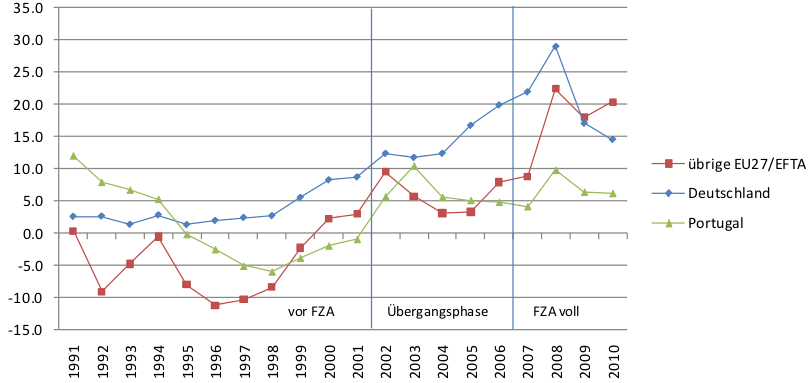
\includegraphics[width=0.9\textwidth]{images/Zuwanderungssaldo_Bericht_2.png}
%	\end{center}
%	\caption{Verlauf der Zuwanderung nach Herkunftsländern in Tausend \cite[S. 18]{ADMIN:Bericht}}
%	\label{fig:zuwanderungsaldi}
%\end{figure*}


\section{Code Generation}

Die Zielplattform des generierten Codes ist die Java Virtual Machine \cite{ORACLE:JVM}. Daher
wird Java Bytecode generiert. Dies kann mit den selben Prinzipien angegangen werden, welche auch
bei der Generierung von Maschinen Code oder Code für die im Unterricht zur Verfügung gestellte 
VM gelten. Da die JVM jedoch von Beginn an auf die Sprache Java zugeschnitten wurde, gibt es bei
der Abbildung eines IML Programmes auf die Struktur eines JVM Programmes einige Spezialitäten, 
auf welche in diesem Abschnitt eingegangen wird.

\subsection {Strukturierung}

Die JVM ist wie die Sprache Java objektorientiert aufgebaut. Aus diesem Grund muss ein 
IML Programm auf die Klassenstruktur der JVM abgebildet werden. In diesem Abschnitt wird 
anhand des Beispielprogramms aus Listing \ref{lst:outtest} die Abbildung auf eine JVM Klasse
erläutert. Dieses IML Programm wird zu einer Klasse, welcher der Klassendeklaration in Listing 
\ref{lst:outtest_class} entspricht. Dabei wurde folgende Abbilung gewählt:

\begin{itemize}
    \item \textbf{Program}: Ein IML Programm wird auf eine Klasse mit gleichem Namen abgebildet.
                            Um die Kompatibilität mit andern JVM Sprachen zu gewährleisten werden die globalen
                            Variablen im Konstruktor mit Defaultwerten initialisiert. Die Klasse wurde als final 
                            gekennzeichnet, um späteres überschreiben von Methoden zu verhindern.
    \item \textbf{Globale Variablen}: Globale Variablen werden zu privaten Feldern der Klasse des Programms.
    \item \textbf{Program Body}: Die Commands des IML Programms werden zu einer neuen Funktion der Klasse,
                                 welche den Namen der Klasse hat, kompiliert. Der Vorteil im Gegensatz zum 
                                 direkten kompilieren in die main Methode liegt darin, dass die globalen Variablen 
                                 und Routinen nicht \textit{static} sein müssen und so mehrere Instanzen des 
                                 IML Programms in der selben VM aktiv sein können, ohne Zustand teilen zu müssen. 
                                 Dies würde es auch erlauben Bibliotheksfunktionen in IML zu entwickeln und 
                                 in anderen JVM Sprachen zu verwenden.
    \item \textbf{Routinen}: Routinen werden zu Funktionen der Klasse. Wenn keine out-Parameter verwendet
                             werden entsprechen diese Funktionen normalen JVM Funktionen und stehen ohne 
                             spezielle Konventionen an den Aufruf zur Verfügung. Wie out-Parameter abgebildet 
                             werden ist im nächsten Abschnitt erläutert.
    \item \textbf{Eintrittpunkt}: Falls die JVM eine Klasse ausführen will, so ruft sie die Funktion \textbf{main}
                                  auf. Daher wird ebenfalls eine solche generiert, welche eine neue Instanz der 
                                  Klasse erzeugt und die Methode mit dem gleichen Namen der Klasse ausführt.
\end{itemize}
\vspace{0.5cm}
\begin{lstlisting}[caption=Laden eines Int-Wertes in zwei Speicherstellen über out Parameter,label={lst:outtest}]
program outtest
global
    proc loadTwice(ref i: int32, out ref a: int32, out ref b: int32)
    requires[ i > 0 : exampleCondition ]
    ensures[ a = old(i), b = old(i) ]
    {
        a init := i;
        b init := i
    };
    a: int32;
    b: int32;
    var v: int32
{
    v init := 12;
    call loadTwice(v, a init, b init);
    ! a;
    ! b
}
\end{lstlisting}

\begin{lstlisting}[caption=Struktur der Klasse,language=Java,label={lst:outtest_class}]
public final class outtest {
    public void loadTwice(int, int[], int[]);
    public outtest();
    public void outtest();
    public static void main(java.lang.String[]);
}
\end{lstlisting}


\subsection {Parameterübergabe}

IML unterstüzt ein sehr ausgefeiltes Handling von Parameterwerten. Die JVM jedoch erlaubt 
das Übergeben von Parametern lediglich \textit{by-value}. Zudem ist es in IML möglich 
festzulegen ob ein Parameter ein Eingabeparameter, Ausgabeparameter oder beides ist. Auch hier 
erlaubt die JVM lediglich Eingabeparameter. Um Parameter von IML vollständig abbilden zu können 
werden auch \textit{ref} Parameter wie \textit{copy} Parameter behandelt. \textit{out}-Parameter 
können so jedoch nicht realisiert werden, da die JVM dafür Referenzen auf primitive Typen 
unterstützen müsste. Um nun das Schreiben von Informationen in den Speicherbereich des Aufrufers
zu erlauben, könnte eine Hilfsklasse (z.B. IntRef) erzeugt werden. Dies würde jedoch eine 
Abhängigkeit zu dieser Klasse für den generierten Code und jeden, der diesen Benutzen möchte, 
zur Folge haben. Dies kann umgangen werden, wenn der entsprechende Parameter in ein Array mit
der Länge 1 umgewandelt wird. So können \textit{out} Parameter auf der JVM elegant implementiert werden.
Dies bedeutet für den Aufrufer jedoch mehr Aufwand, da er zunächst für jeden \textit{out} Parameter 
ein neues Array erzeugen und den zu übergebenden Wert(im Falle von \textit{inout}) hineinkopieren muss. 
Im Anschluss an den Methodenaufruf muss der Wert im Array wieder an die Speicherstelle des ursprünglichen 
Wertes kopiert werden. Für den Aufgerufenen fällt jedoch keinerlei Zusatzaufwand an, wie in Listing 
\ref{lst:loadtwice_code} zu sehen ist.
\newline

\begin{lstlisting}[caption=Bytecode der loadTwice Prozedur ohne conditions,label={lst:loadtwice_code}]
public void loadTwice(int, int[], int[]);
    flags: ACC_PUBLIC
    Code:
      stack=3, locals=4, args_size=4
        0: aload_2          // Laden des 2. Parameters auf Stack (Array Referenz)
        1: iconst_0         // Laden von 0 auf den Stack (Pos in Array)
        2: iload_1          // Laden des ersten Parameters auf Stack (zu speichernder Wert)
        3: iastore          // Speichern (int array store)
        4: aload_3       
        5: iconst_0      
        6: iload_1       
        7: iastore       
        8: return
\end{lstlisting}


\subsection{Pre-/Postconditions}

Für das Umsetzen der Pre-/Postconditions kann gewöhnlicher Code generiert werden. Falls eine der Conditions
jedoch fehlschlägt, muss die Programmausführung unterbrochen werden. Da Java bereits ein Konstruktr für 
Assertions unterstützt, gibt es bereits in der Standartbibliothek die AssertionError Exception.
Diese kann auch für die Conditions in IML verwendet werden, wobei das Label der Condition, falls vorhanden,
als Exception Message verwendet wird.
\newline

\begin{lstlisting}[caption=Bytecode der loadTwice Prozedur mit precondition,label={lst:loadtwice_code_precond}]
public void loadTwice(int, int[], int[]);
    flags: ACC_PUBLIC
    Code:
      stack=3, locals=4, args_size=4
         0: iload_1       
         1: bipush        0
         3: if_icmple     10
         6: iconst_1      
         7: goto          11
        10: iconst_0      
        11: ifeq          17
        14: goto          27              // Weiter mit normalem Code
        17: new           #9              // class java/lang/AssertionError
        20: dup         
        21: ldc           #11             // Laden der String Konstante "exampleCondition"
        23: invokespecial #15             // Method java/lang/AssertionError."<init>"
        26: athrow                        // Werfen der Exception
        27: aload_2       
        28: iconst_0      
        29: iload_1       
        30: iastore       
        31: aload_3       
        32: iconst_0      
        33: iload_1       
        34: iastore       
        35: return  
\end{lstlisting}

\subsubsection{Speichern des Preexecution States}

Der Preexecution State wird im Stack Frame der Methode als lokale Variable gespeichert. Wenn nun 
die Postcondtitions ausgewertet werden, wird im Falle eines Calls der \textit{old} Funktion der Wert 
an der entsprechenden Position der lokalen Variable geliefert.
\newline
\begin{lstlisting}[caption=Bytecode der loadTwice Prozedur mit postcondition mit Zugriff auf old State. Damit der Code etwas Übersichtlicher ist\, wurde nur die erste Postcondtition kompiliert.,label={lst:loadtwice_code_old}]
public void loadTwice(int, int[], int[]);
    flags: ACC_PUBLIC
    Code:
      stack=3, locals=5, args_size=4
         0: iload_1                 // Expression in old(i) -> i 
         1: istore        4         // Speichern an lokalem variablen Index 4
         3: aload_2                 // Normaler Code
         4: iconst_0      
         5: iload_1       
         6: iastore       
         7: aload_3       
         8: iconst_0      
         9: iload_1       
        10: iastore       
        11: aload_2       
        12: iconst_0      
        13: iaload        
        14: iload         4         // Zuvor gespeicherter Wert laden
        16: if_icmpne     23
        19: iconst_1      
        20: goto          24
        23: iconst_0      
        24: ifeq          30
        27: goto          38
        30: new           #9        // class java/lang/AssertionError
        33: dup           
        34: invokespecial #13       // Method java/lang/AssertionError."<init>":()V
        37: athrow        
        38: return
\end{lstlisting}



\section{Vergleich mit anderen Programmiersprachen}
In diesem Abschnitt wird der gewählte Entwurf mit Implementierungen
für andere Sprachen verglichen.

\subsection{Java / C(++)}
Die meistverwendeten Sprachen Java, sowie C(++) enthalten keine Unterstützung des Compilers 
zur Definition von pre-/postconditions auf Methoden. Jedoch gibt es die Möglichkeit 
über \textit{Assertions} Bedingungen im Code zu definieren, welche zu einem Programmabbruch führen.
Darüber hat ein Programmierer die Möglichkeit conditions zu formulieren. Diese können jedoch über weite
Teile des Quellcodes verteilt sein und es ist für einen anderen Programmierer nicht 
sofort ersichtlich welche pre-/postconditions daraus abgeleitet werden können. Im speziellen 
Fall von Java ist es zudem so, dass die Ausführung von Assertions defaultmässig nicht aktiviert 
ist. Daher ist der Nutzen solcher Assertions leider nur gering. Da diese Sprachen jedoch 
sehr weit verbreitet sind haben sich zahlreiche Frameworks entwickelt, welche es erlauben
zusätzliche Bedingungen an Methodenaufrufe zu knüpfen. Diese sind jedoch nicht im Compiler integriert
und haben sich daher auch nicht weit verbreitet.

\subsection{C\# (.NET Framework)}

Für die Common Language Runtime (CLR) von Microsoft gilt eigentlich dasselbe wie für die Sprachen 
Java und C(++). Es muss jedoch erwähnt werden, dass von Microsoft Research Tools entwickelt wurden, 
die in dieser Form in keiner der obengennanten Sprachen umgesetzt wurden. Das Framework 
\textit{Code Contracts} ermöglicht es dem Programmierer über statische Methodenaufrufe 
conditions(oder eben contracts) zu formulieren (ähnlich wie Assertions). 
Danach ist es dem Framework möglich, daraus sowohl Laufzeitchecks als auch 
Dokumentationsdateien zu generieren. Viel interessanter ist jedoch die Möglichkeit einen 
statischen Checker zu benutzen, welcher Contracts bereits zur compile-time überprüfen 
kann \cite{MS:StaticAnalysis}. Dies geht viel weiter als unsere Imeplementirung für IML, 
ist jedoch nicht direkt in der Sprache enthalten.

\subsection{Eiffel}
Die Sprache Eiffel enthält sehr ähnliche Implementierung wie die von uns für IML gewählte. Durch
die objektorientierte Natur von Eiffel unterstützt sie zusätzlich Klasseninvarianten, wie auch die
Vererbung von conditions. Den Zugriff auf pre-execution State von Variablen wir über das 
Keyword \textit{old} ermöglicht.

\subsection{D}
Die Sprache D\cite{D:Main}, welche C++ weiterentwickeln soll, ermöglicht es sowohl Klassen-Invarianten,
als auch conditions auf der Ebene eines Statements zu definieren. Da auch diese Sprache objektorientiert 
ist, wurden Klasseninvarianten implementiert. Es ist jedoch nicht möglich innerhalb der Postcondition 
auf den Zustand von Variablen vor der Ausführung des bodys zuzugreifen.\newline

\begin{lstlisting}[caption=Beispiel in D]
in 
{ 
    assert(x >= 0);
} 
out (result) 
{
    assert((result * result) <= x && (result+1) * (result+1) >= x);
} 
body
{
    ... code ...
}
\end{lstlisting}

\subsection{Ada}
Ada erlaubt die Definition von pre-postconditions auf Ebene von Prozeduren/Funktionten und Subtypen 
seit der Version 2012. Subtypen sind
dabei bereits eine Art von Einschränkung, welche vom Comiler als Typ aufgefasst werden und daher bereits
bei der Kompilationszeit erkannt werden. Seit Ada 2012 ist es jedoch auch möglich, solche Subtypen 
mit dynamischen und statischen Prädikaten zu versehen. Dabei werden die dynamischen zur Laufzeit 
überprüft, während die statischen viele Überprüfungen bereits zur Kompilationszeit
 durchführen können. Auch 
Ada erlaubt den Zugriff auf Zustand vor der Ausführung der Prozedur. \newline

\begin{lstlisting}[caption=Beispiel in Ada 2012,language=Ada]
procedure Update_Person (P : in out Person)
   with Post => P.Sex = P.Sex'Old 
                and P.Birth_Date = P.Birth_Date'Old;

function Inc(X: Integer) return Integer
   with Pre  => X /= Integer'Last,
        Post => Inc'Result = X'Old+1;
\end{lstlisting}



% Schluss
\section{Zusammenarbeit}

Das Programm zur Generierung der Parsetabelle ohne Erweiterungen wurde uns freundlicherweise 
vom Team 08 (Walther/Martin) zur Verfügung gestellt.

\section{Arbeitsaufteilung}

Der Grossteil des Codes sowie der Dokumentation wurde gemeinsam erarbeitet. Jedoch wurde der 
Initialisierungscheck grösstenteils von Matthias Brun implementiert, während sich Florian Lüscher
mit der Code Generierung beschäftigte.

\section{Erklärung}

Hiermit bestätigen wir die Korrektheit der Angaben und das selbständige Erarbeiten dieser Arbeit
sowie des Codes, sofern nichts anders deklariert wurde.

\hspace{3cm}Florian Lüscher\hspace{5cm}Matthias Brun

%Was noch verbessert werden kann..

%\section{Fazit}

%Welche Erfahrungen wurden gemacht...


\vspace{50pt}

% Bildverzeichnis
%\listoffigures

\vspace{20pt}

% Quellverzeichnis
\bibliographystyle{IEEEtran}
\bibliography{report.bib}

\newpage

\begin{appendix}

\section{Vollständige Grammatik}
\label{sec:fullgrammar}

\lstinputlisting{content/grammar.bnf}

\section{Funktionierende Beispiele}
\label{sec:good_examples}


\section{Nicht funktionierende Beispiele}
\label{sec:bad_examples}


\end{appendix}


\end{document}
